\documentclass[UTF-8,notitlepage,onecolumn,oneside]{article}

%导言区
%--包引用
\usepackage{ctex}
\usepackage{geometry}
\usepackage{setspace}
\usepackage{tabularx}
\usepackage{graphicx}
\usepackage{booktabs}
\usepackage{amsmath}

%--定义字体
\newcommand{\erhaoheiti}{\fontsize{22pt}{\baselineskip}\heiti\selectfont}%二号黑体
\newcommand{\sihaofangsong}{\fontsize{14.1pt}{\baselineskip}\fangsong\selectfont}%四号仿宋
\newcommand{\wuhaosongti}{\fontsize{10.5pt}{\baselineskip}\songti\selectfont}%五号宋体
\newcommand{\wuhaoheiti}{\fontsize{10.5pt}{\baselineskip}\heiti\selectfont}%五号黑体
\newcommand{\sihaoheiti}{\fontsize{14.1pt}{\baselineskip}\heiti\selectfont}%四号黑体
\newcommand{\xiaosihaoheiti}{\fontsize{12.1pt}{\baselineskip}\heiti\selectfont}%小四黑体
\newcommand{\xiaosisongti}{\fontsize{12.1pt}{\baselineskip}\songti\selectfont}%小四黑体
\newcommand{\wuhaotimes}{\fontsize{10.5pt}{\baselineskip}\Times\selectfont}%五号times,用于英文文献
\newcommand{\upcite}[1]{\textsuperscript{\textsuperscript{\cite{#1}}}}
%--部分设置
 \geometry{
	a4paper,
	left=31.8mm,
	right=31.8mm,
	top=25.4mm,
	bottom=25.4mm
	}

%--标题
\title{题目(二号黑体)}
\author{作者(四号仿宋)\\ 上海大学上海电影学院XX专业2019级硕/博士(五号宋体)}
\date{}

%--正文
\begin{document}
	\begin{spacing}{1.5}%1.5倍行距
	\begin{center}
	\begin{erhaoheiti}
		题目(二号黑体)\\
	\end{erhaoheiti}
	\begin{sihaofangsong}
		作者(四号仿宋)\par\par
	\end{sihaofangsong}
	\vspace{0ex}
	\begin{wuhaosongti}
		上海大学上海电影学院XX专业2019级硕/博士(五号宋体)
	\end{wuhaosongti}
	\end{center}
	\end{spacing}
 	\vspace{-3ex}
	\begin{flushleft}
		\setstretch{1.1}
		\wuhaoheiti 摘\quad 要(五号宋体加粗)~
		\wuhaosongti 本文提出了…\upcite{Bilen2016}。该算法基于……。与现有的算法相比,本文的方法易于实现\upcite{Ahad2011},同时实验显示该算法具有更好的计算性能。(100-300字,五号宋体)	\\
		\vspace{-1ex}
		\wuhaoheiti 关键词(五号宋体加粗)~
		\wuhaosongti 算法~~编码~~N维Hilbert曲线~~空间填充曲线	
	\end{flushleft}
	\vspace{-5ex}
	\section{引言\vspace{-0.5ex}}
		\xiaosisongti{关于Hilbert曲线编码生成,有两种实现方法:一个是表\upcite{Sigal2010}驱动方法,一个是计算的方法。表驱动的一个最大的缺点就是它的空间复杂度很高。(正文:小四号宋体)}
		\vspace{-1em}
	\section{分析Hilbert曲线\vspace{-0.5em}}
	\subsection{Hilbert曲线的定义\vspace{-0.5em}}
		首先,用$R^n$来表示N维空间。用$X_n,…,X_2,X_1$来表示N维空间$R^n$的N个维。把从N维空间坐标转换成的一维空间坐标值叫做Hilbert码,记为:\textbf{H-code}。(正文:小四号宋体)
		\begin{figure}[htbp]
		\centering
		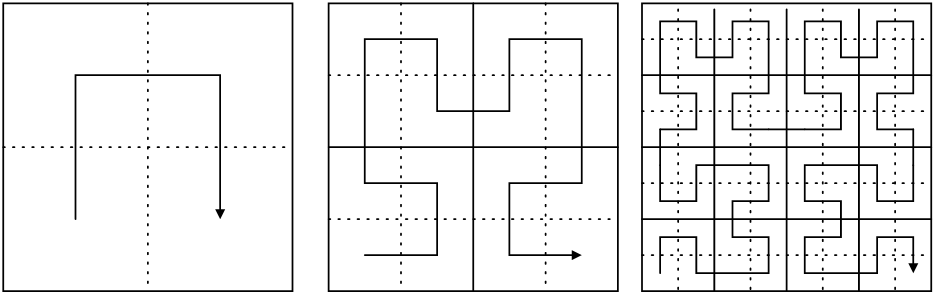
\includegraphics[scale=0.8]{pic.png}
		\vspace{-2ex}
		\caption{Hilbert曲线}
		\label{fig:Hilbert}
		\end{figure}
	\vspace{-4ex}
	\begin{table}[htbp]
		\caption{3维forward扫描单元}
		\vspace{1ex}
		\centering
		\begin{tabular}{llll}
			\toprule
			x1 & x2 & x3 & x4     \\ 
			\midrule[0.25ex]
			0  & 1  & 1  & 010    \\
			1  & 0  & 0  & 111    \\
			1  & 0  & 1  & 110    \\ 
			1  & 1  & 0  & 100    \\ 
			\bottomrule
		\end{tabular}
	\end{table}
	\vspace{-3ex}
	\begin{equation}\label{eq:1}
		i\hbar \frac{\partial}{\partial t}\Psi \left( r,t \right) =\hat{H}\Psi \left( r,t \right)
	\end{equation}
		
	\begin{spacing}{1}
		\small
	\bibliographystyle{plain}
	\bibliography{ref}
	\end{spacing}

\end{document}
